\documentclass[12pt,a4paper]{article}

\usepackage[a4paper,text={16.5cm,25.2cm},centering]{geometry}
\usepackage{lmodern}
\usepackage{amssymb,amsmath}
\usepackage{bm}
\usepackage{graphicx}
\makeatletter
\def\maxwidth{\ifdim\Gin@nat@width>\linewidth\linewidth\else\Gin@nat@width\fi}
\makeatother
\setkeys{Gin}{width=\maxwidth,keepaspectratio}
\usepackage{float}

\usepackage{microtype}
\usepackage{hyperref}
\setlength{\parindent}{0pt}
\setlength{\parskip}{1.2ex}

\hypersetup
       {   pdfauthor = { Gandhi Alexis Sinhue Contreras Torres },
           pdftitle={ DSP Homework 6 },
           colorlinks=TRUE,
           linkcolor=black,
           citecolor=blue,
           urlcolor=blue
       }

\title{ DSP Homework 6 }

\author{ Gandhi Alexis Sinhue Contreras Torres }

\date{ 10/07/2026 }

\usepackage{upquote}
\usepackage{listings}
\usepackage{xcolor}
\lstset{
    basicstyle=\ttfamily\footnotesize,
    upquote=true,
    breaklines=true,
    breakindent=0pt,
    keepspaces=true,
    showspaces=false,
    columns=fullflexible,
    showtabs=false,
    showstringspaces=false,
    escapeinside={(*@}{@*)},
    extendedchars=true,
}
\newcommand{\HLJLt}[1]{#1}
\newcommand{\HLJLw}[1]{#1}
\newcommand{\HLJLe}[1]{#1}
\newcommand{\HLJLeB}[1]{#1}
\newcommand{\HLJLo}[1]{#1}
\newcommand{\HLJLk}[1]{\textcolor[RGB]{148,91,176}{\textbf{#1}}}
\newcommand{\HLJLkc}[1]{\textcolor[RGB]{59,151,46}{\textit{#1}}}
\newcommand{\HLJLkd}[1]{\textcolor[RGB]{214,102,97}{\textit{#1}}}
\newcommand{\HLJLkn}[1]{\textcolor[RGB]{148,91,176}{\textbf{#1}}}
\newcommand{\HLJLkp}[1]{\textcolor[RGB]{148,91,176}{\textbf{#1}}}
\newcommand{\HLJLkr}[1]{\textcolor[RGB]{148,91,176}{\textbf{#1}}}
\newcommand{\HLJLkt}[1]{\textcolor[RGB]{148,91,176}{\textbf{#1}}}
\newcommand{\HLJLn}[1]{#1}
\newcommand{\HLJLna}[1]{#1}
\newcommand{\HLJLnb}[1]{#1}
\newcommand{\HLJLnbp}[1]{#1}
\newcommand{\HLJLnc}[1]{#1}
\newcommand{\HLJLncB}[1]{#1}
\newcommand{\HLJLnd}[1]{\textcolor[RGB]{214,102,97}{#1}}
\newcommand{\HLJLne}[1]{#1}
\newcommand{\HLJLneB}[1]{#1}
\newcommand{\HLJLnf}[1]{\textcolor[RGB]{66,102,213}{#1}}
\newcommand{\HLJLnfm}[1]{\textcolor[RGB]{66,102,213}{#1}}
\newcommand{\HLJLnp}[1]{#1}
\newcommand{\HLJLnl}[1]{#1}
\newcommand{\HLJLnn}[1]{#1}
\newcommand{\HLJLno}[1]{#1}
\newcommand{\HLJLnt}[1]{#1}
\newcommand{\HLJLnv}[1]{#1}
\newcommand{\HLJLnvc}[1]{#1}
\newcommand{\HLJLnvg}[1]{#1}
\newcommand{\HLJLnvi}[1]{#1}
\newcommand{\HLJLnvm}[1]{#1}
\newcommand{\HLJLl}[1]{#1}
\newcommand{\HLJLld}[1]{\textcolor[RGB]{148,91,176}{\textit{#1}}}
\newcommand{\HLJLs}[1]{\textcolor[RGB]{201,61,57}{#1}}
\newcommand{\HLJLsa}[1]{\textcolor[RGB]{201,61,57}{#1}}
\newcommand{\HLJLsb}[1]{\textcolor[RGB]{201,61,57}{#1}}
\newcommand{\HLJLsc}[1]{\textcolor[RGB]{201,61,57}{#1}}
\newcommand{\HLJLsd}[1]{\textcolor[RGB]{201,61,57}{#1}}
\newcommand{\HLJLsdB}[1]{\textcolor[RGB]{201,61,57}{#1}}
\newcommand{\HLJLsdC}[1]{\textcolor[RGB]{201,61,57}{#1}}
\newcommand{\HLJLse}[1]{\textcolor[RGB]{59,151,46}{#1}}
\newcommand{\HLJLsh}[1]{\textcolor[RGB]{201,61,57}{#1}}
\newcommand{\HLJLsi}[1]{#1}
\newcommand{\HLJLso}[1]{\textcolor[RGB]{201,61,57}{#1}}
\newcommand{\HLJLsr}[1]{\textcolor[RGB]{201,61,57}{#1}}
\newcommand{\HLJLss}[1]{\textcolor[RGB]{201,61,57}{#1}}
\newcommand{\HLJLssB}[1]{\textcolor[RGB]{201,61,57}{#1}}
\newcommand{\HLJLnB}[1]{\textcolor[RGB]{59,151,46}{#1}}
\newcommand{\HLJLnbB}[1]{\textcolor[RGB]{59,151,46}{#1}}
\newcommand{\HLJLnfB}[1]{\textcolor[RGB]{59,151,46}{#1}}
\newcommand{\HLJLnh}[1]{\textcolor[RGB]{59,151,46}{#1}}
\newcommand{\HLJLni}[1]{\textcolor[RGB]{59,151,46}{#1}}
\newcommand{\HLJLnil}[1]{\textcolor[RGB]{59,151,46}{#1}}
\newcommand{\HLJLnoB}[1]{\textcolor[RGB]{59,151,46}{#1}}
\newcommand{\HLJLoB}[1]{\textcolor[RGB]{102,102,102}{\textbf{#1}}}
\newcommand{\HLJLow}[1]{\textcolor[RGB]{102,102,102}{\textbf{#1}}}
\newcommand{\HLJLp}[1]{#1}
\newcommand{\HLJLc}[1]{\textcolor[RGB]{153,153,119}{\textit{#1}}}
\newcommand{\HLJLch}[1]{\textcolor[RGB]{153,153,119}{\textit{#1}}}
\newcommand{\HLJLcm}[1]{\textcolor[RGB]{153,153,119}{\textit{#1}}}
\newcommand{\HLJLcp}[1]{\textcolor[RGB]{153,153,119}{\textit{#1}}}
\newcommand{\HLJLcpB}[1]{\textcolor[RGB]{153,153,119}{\textit{#1}}}
\newcommand{\HLJLcs}[1]{\textcolor[RGB]{153,153,119}{\textit{#1}}}
\newcommand{\HLJLcsB}[1]{\textcolor[RGB]{153,153,119}{\textit{#1}}}
\newcommand{\HLJLg}[1]{#1}
\newcommand{\HLJLgd}[1]{#1}
\newcommand{\HLJLge}[1]{#1}
\newcommand{\HLJLgeB}[1]{#1}
\newcommand{\HLJLgh}[1]{#1}
\newcommand{\HLJLgi}[1]{#1}
\newcommand{\HLJLgo}[1]{#1}
\newcommand{\HLJLgp}[1]{#1}
\newcommand{\HLJLgs}[1]{#1}
\newcommand{\HLJLgsB}[1]{#1}
\newcommand{\HLJLgt}[1]{#1}


\begin{document}

\maketitle

\section{Homework 6}
This document contains the solutions for DSP Homework 6, on the $z$-transform (Mitra, 4th ed., Chapter 6). For each problem the statement is given, followed by a short note naming the rule used and where it is found in the book, and then the hand-written derivation.

All page numbers refer to the printed pages of Chapter 6. The rules used throughout are: the definition of the $z$-transform (Sec. 6.1, p. 277), the standard transform pairs (Table 6.1, p. 281), the rational form of Eq. (6.13) (Sec. 6.2, p. 281), the ROC rules for right- and left-sided sequences (Sec. 6.3, pp. 283-285), the inverse transform by partial-fraction expansion (Sec. 6.4.3, p. 291) and by power-series expansion (Sec. 6.4.5, p. 295), the transform properties of Table 6.2 (Sec. 6.5, p. 297), the transfer function of a difference equation (Sec. 6.7.2, p. 309), the frequency response (Sec. 6.7.3, p. 312), and the stability condition in terms of pole locations (Sec. 6.7.5, p. 315).

\subsection{6.8(a) | ROC of the z-transform of each sequence}
Determine the ROC of the $z$-transform of each of the following sequences:

(i) $x_1[n] = (0.2)^n \mu[n+1]$

(ii) $x_2[n] = (0.6)^n \mu[n-2]$

(iv) $x_4[n] = (-0.5)^n \mu[-n-3]$

\emph{Method.} Apply the definition (Sec. 6.1, p. 277) and recall that the geometric series $\sum_{k \ge 0} a^k$ converges if and only if $|a| < 1$; this is what produces every ROC. Then use the ROC shape rules (Sec. 6.3): a right-sided sequence gives an exterior, with $z = \infty$ included only if the sequence is causal (p. 284); a left-sided sequence gives an interior, with $z = 0$ included only if the sequence is anticausal (p. 285).

\begin{figure}[H]
\centering
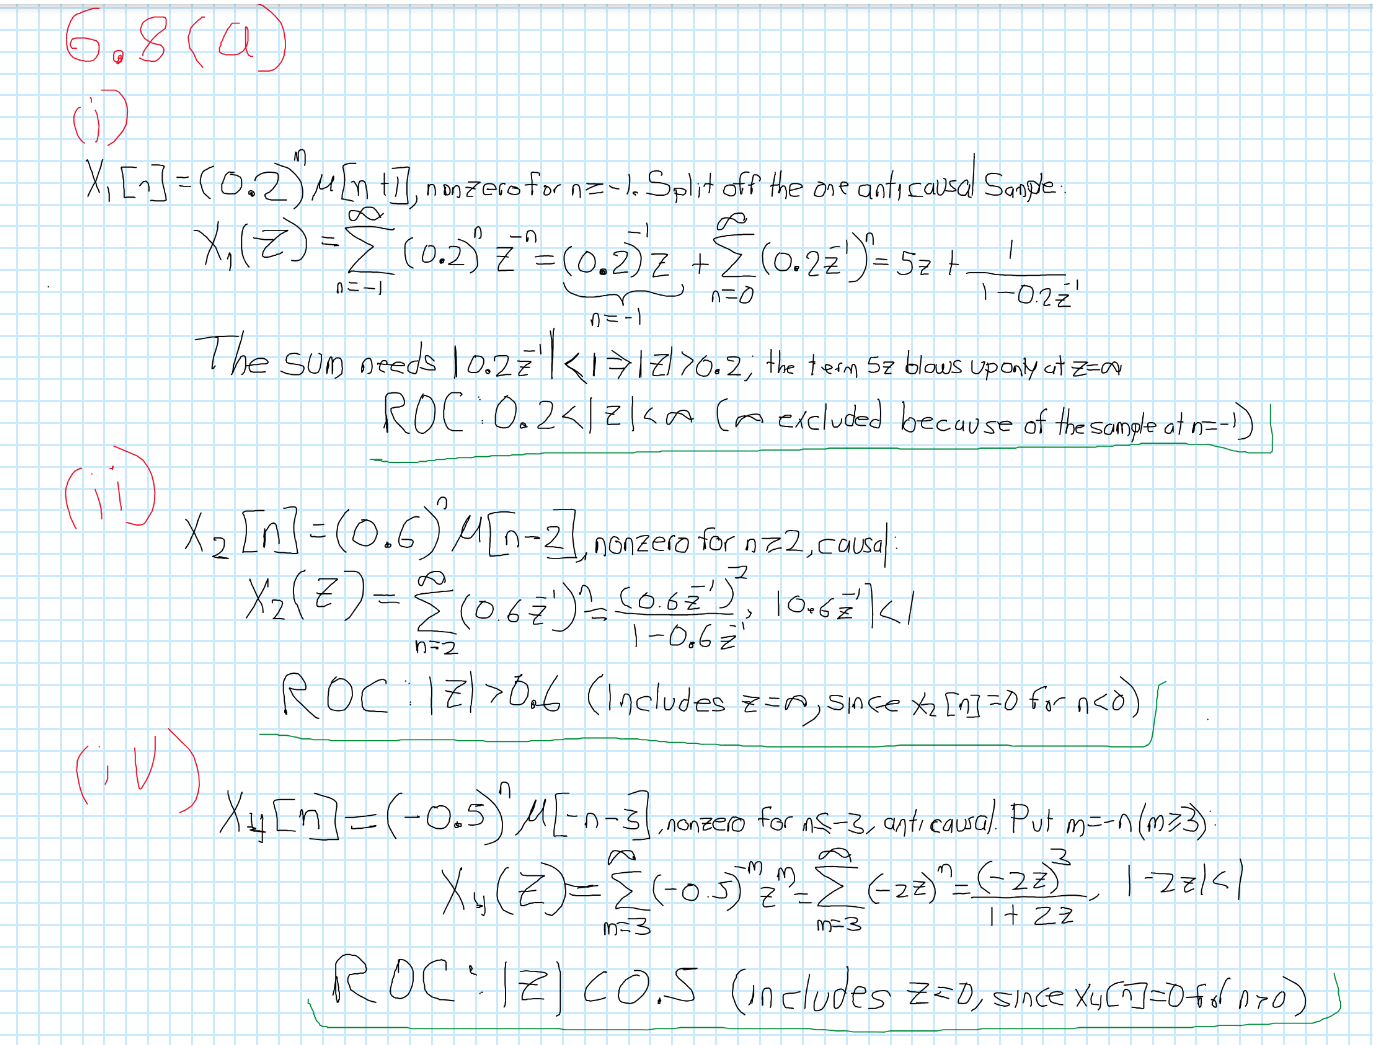
\includegraphics{figures/6_8a.png}
\caption{Hand solution, Problem 6.8(a)}
\end{figure}


\subsection{6.8(b) | ROC of the sums}
From the ROCs determined in Part (a), determine the ROCs of the following sequences:

(i) $y_1[n] = x_1[n] + x_2[n]$

(iii) $y_3[n] = x_1[n] + x_4[n]$

(v) $y_5[n] = x_2[n] + x_4[n]$

\emph{Method.} Linearity (Table 6.2, p. 297): the ROC of $\alpha g[n] + \beta h[n]$ \emph{includes} $R_g \cap R_h$. Here the poles $0.2$, $0.6$ and $0.5$ are distinct, so there is no pole-zero cancellation and the ROC is exactly the intersection. Note that in one of the three cases the intersection is empty.

\begin{figure}[H]
\centering
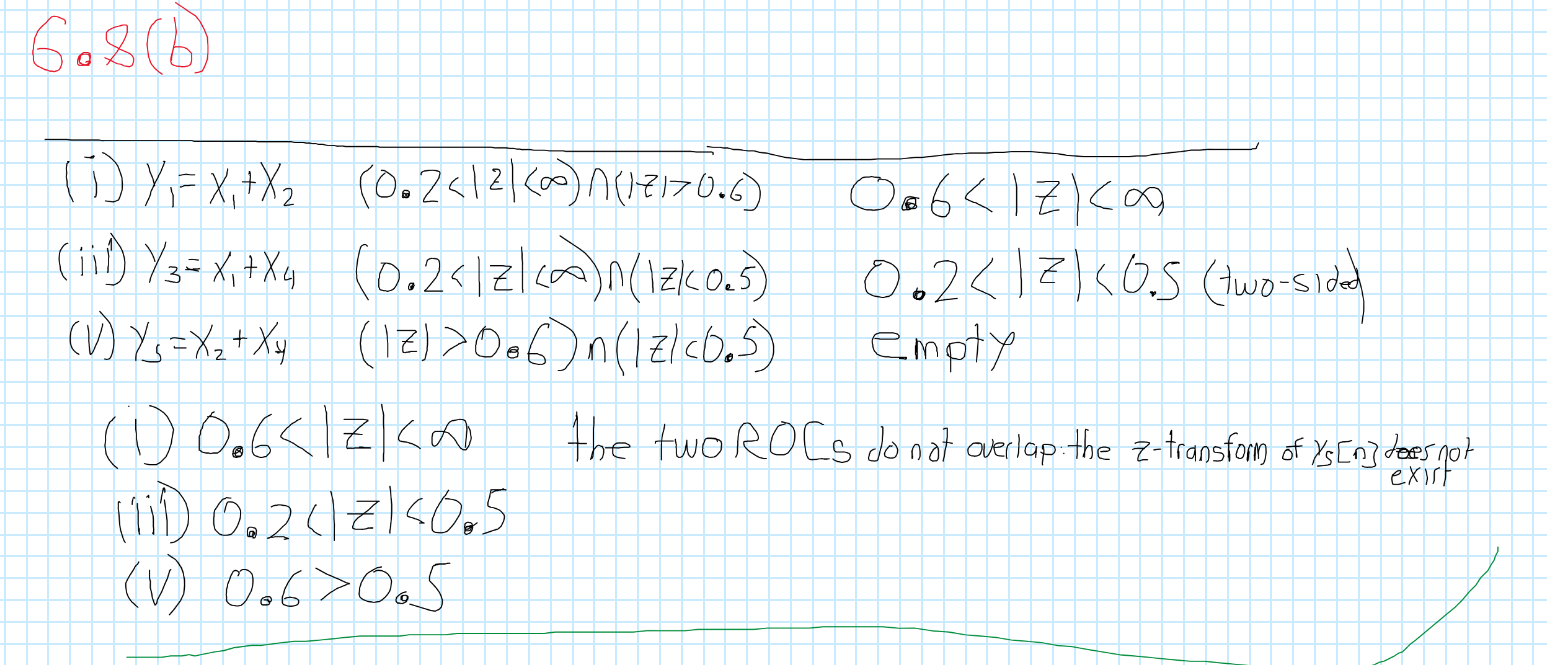
\includegraphics{figures/6_8b.png}
\caption{Hand solution, Problem 6.8(b)}
\end{figure}


\subsection{6.11 | z-transform and ROC by repeated differentiation}
Determine the $z$-transform and the corresponding ROC of the following sequences:

(a) $y_1[n] = n^2 \alpha^n \mu[n]$

(b) $y_2[n] = n^3 \alpha^n \mu[n]$

(c) $y_3[n] = \frac{(n+1)(n+2)}{2} \alpha^n \mu[n]$

\emph{Method.} Start from the base pair $\alpha^n \mu[n] \leftrightarrow 1/(1 - \alpha z^{-1})$, $|z| > |\alpha|$ (Table 6.1, p. 281), and apply the differentiation property $n\, g[n] \leftrightarrow -z\, dG(z)/dz$ (Table 6.2, p. 297), which leaves the ROC unchanged. Substituting $u = \alpha z^{-1}$ turns the operator $-z\, d/dz$ into $u\, d/du$, which makes the algebra much shorter. Part (c) follows from differentiating the geometric series twice in $u$.

\begin{figure}[H]
\centering
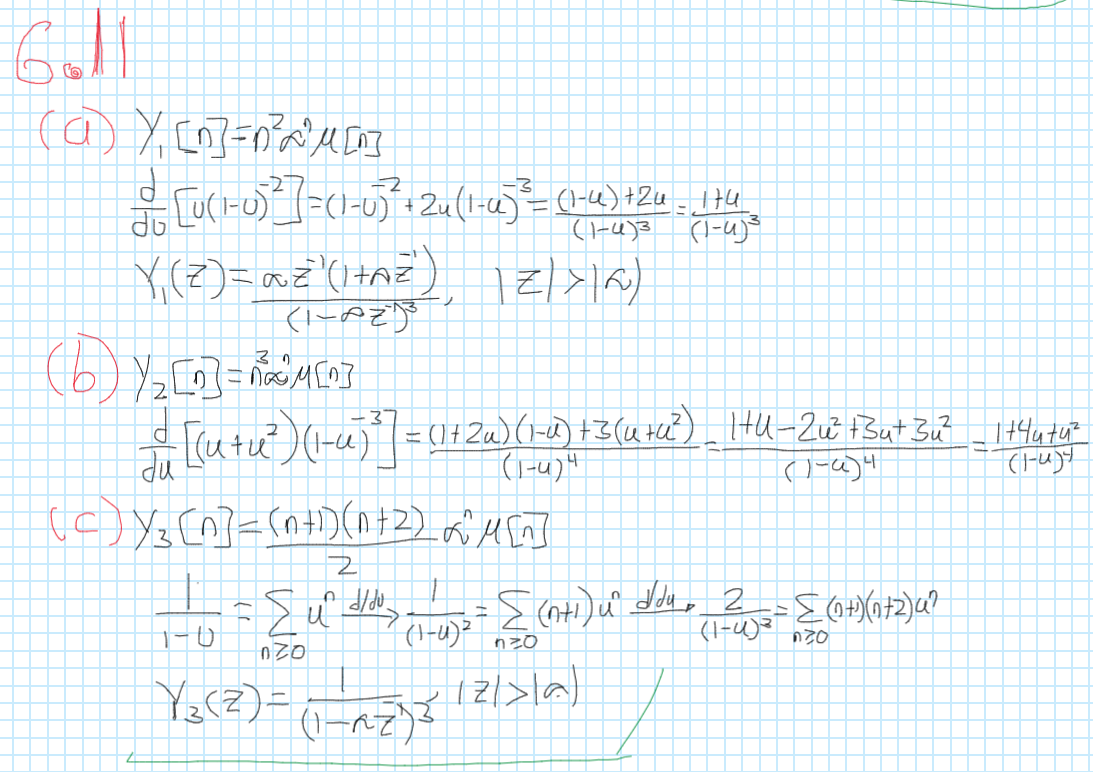
\includegraphics{figures/6_11.png}
\caption{Hand solution, Problem 6.11}
\end{figure}


\subsection{6.14 | z-transform of the cross-correlation}
Let the $z$-transforms of the sequences $x[n]$ and $y[n]$ be denoted by $X(z)$ and $Y(z)$, respectively, with $R_x$ and $R_y$ denoting their respective ROCs. Determine the expression for the $z$-transform of the cross-correlation sequence $r_{xy}[\ell]$ in terms of $X(z)$ and $Y(z)$, and its ROC in terms of $R_x$ and $R_y$. Using this result, determine the $z$-transform $R_{xx}(z)$ of the autocorrelation sequence $r_{xx}[\ell]$ of the causal sequence $x[n] = \alpha^n \mu[n]$, $0 < |\alpha| < 1$, and then determine the expression for the autocorrelation sequence $r_{xx}[\ell]$ by applying the inverse $z$-transform to $R_{xx}(z)$.

\emph{Method.} First write the correlation as a convolution with a reversed sequence, $r_{xy}[\ell] = (x \circledast \tilde{y})[\ell]$ where $\tilde{y}[n] = y[-n]$. Then apply the convolution theorem together with the time-reversal property $g[-n] \leftrightarrow G(1/z)$, ROC $1/R_g$ (both Table 6.2, p. 297). For the inverse, clear $z^{-1}$ first and expand $R_{xx}(z)/z$ by partial fractions (Sec. 6.4.3, p. 291), assigning each term to the correct side of the annulus.

\begin{figure}[H]
\centering
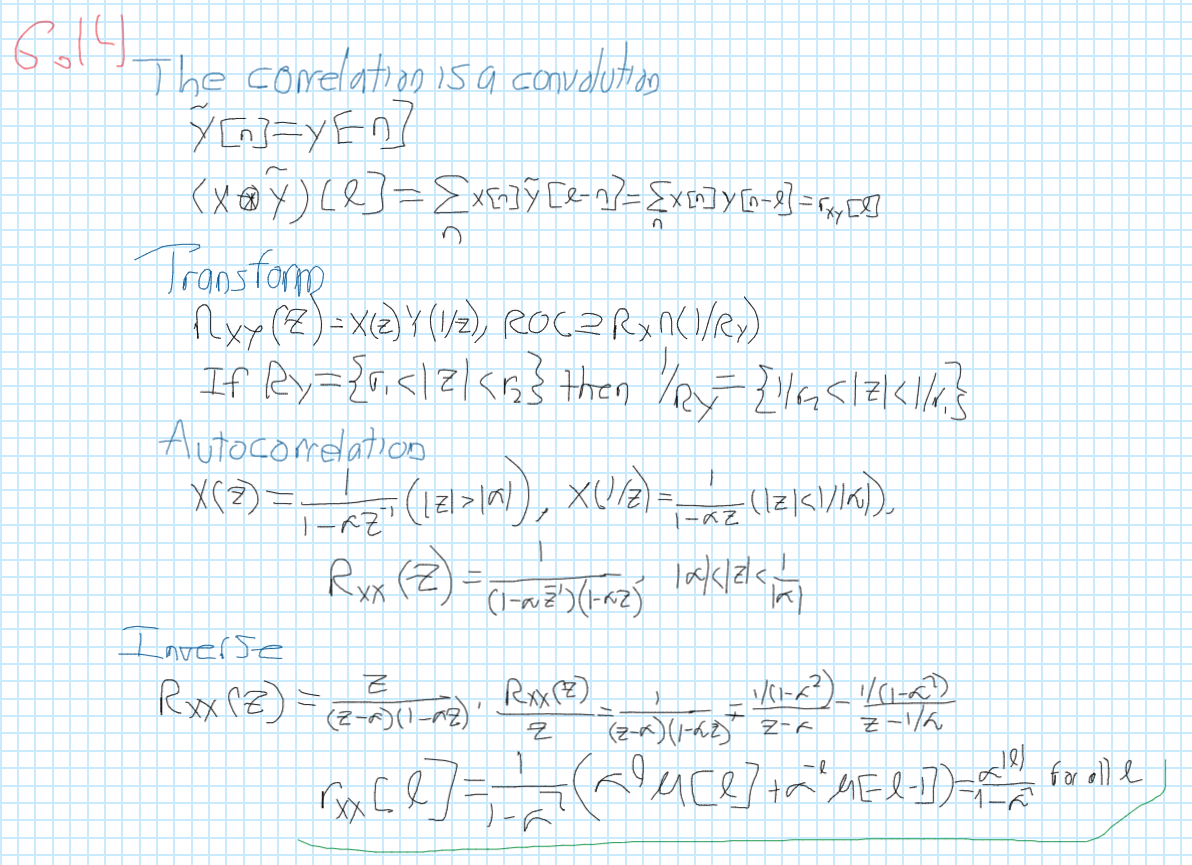
\includegraphics{figures/6_14.png}
\caption{Hand solution, Problem 6.14}
\end{figure}


\subsection{6.23 | z-transform of the Fibonacci sequence}
Determine the $z$-transform $F(z)$ of the Fibonacci sequence $\{f[n]\}$ of Problem 4.39. Evaluate the inverse $z$-transform of $F(z)$.

Recall from Problem 4.39 that $f[n] = f[n-1] + f[n-2]$ for $n \ge 2$, with $f[0] = 0$ and $f[1] = 1$, and $f[n] = 0$ for $n < 0$.

\emph{Method.} The recursion alone does not carry the initial conditions, so first rewrite it as a single equation valid for every $n$ by driving it with an impulse, $f[n] = f[n-1] + f[n-2] + \delta[n-1]$, and verify this at $n = 0$ and $n = 1$. Then apply linearity and the time-shifting property (Table 6.2, p. 297). The sequence is causal, so the ROC is the exterior of the outermost pole (Sec. 6.3, p. 284). Invert by partial fractions (Sec. 6.4.3, p. 291); the result is Binet's formula.

\begin{figure}[H]
\centering
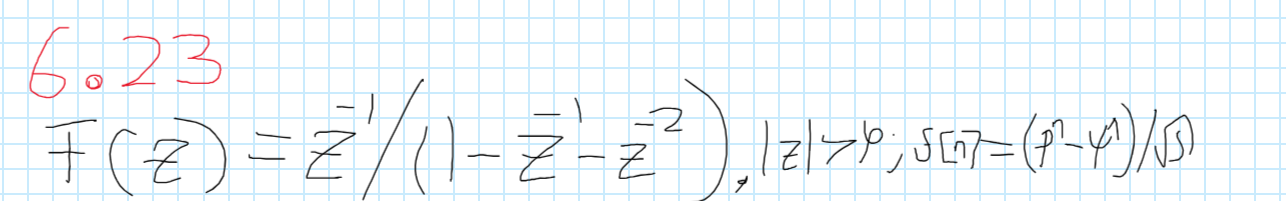
\includegraphics{figures/6_23.png}
\caption{Hand solution, Problem 6.23}
\end{figure}


\subsection{6.30 | Inverse z-transforms of logarithms}
Determine the inverse $z$-transforms of the following $z$-transforms:

(a) $X_1(z) = \log(1 - \alpha z^{-1})$, $|z| > |\alpha|$

(b) $X_2(z) = \log\left(\frac{\alpha - z^{-1}}{\alpha}\right)$, $|z| > 1/|\alpha|$

\emph{Method.} Use the power-series method (Sec. 6.4.5, p. 295): the Laurent expansion of $X(z)$ on its ROC is unique, so matching the coefficients of $z^{-n}$ is a valid inverse transform. The series needed is $\log(1 - w) = -\sum_{k \ge 1} w^k / k$, valid for $|w| < 1$, and the stated ROC is exactly that convergence condition. For part (b), simplify the argument first: $(\alpha - z^{-1})/\alpha = 1 - (1/\alpha) z^{-1}$, so it is part (a) with $\alpha$ replaced by $1/\alpha$. The result of (a) can be checked independently with the differentiation property (Table 6.2, p. 297).

\begin{figure}[H]
\centering
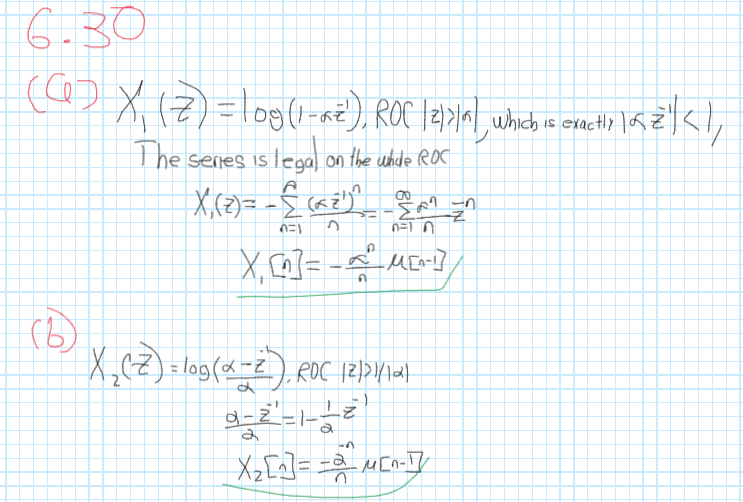
\includegraphics{figures/6_30.png}
\caption{Hand solution, Problem 6.30}
\end{figure}


\subsection{6.31 | p0/d0 equals the sum of the residues}
Consider the $z$-transform $G(z)$ of Eq. (6.13), with $M < N$. If $G(z)$ has only simple poles, show that $p_0/d_0$ is equal to the sum of the residues in the partial-fraction expansion of $G(z)$.

\emph{Method.} Three assumptions do the work. $M < N$ means the partial-fraction expansion has no polynomial (FIR) part; simple poles mean every term is first order with one residue each; and $d_0 \neq 0$ means $G(\infty)$ is finite. With those, the expansion is $G(z) = \sum_{\ell} \rho_\ell / (1 - \lambda_\ell z^{-1})$ (Sec. 6.4.3, p. 291). The proof is then a single move: evaluate both this expansion and Eq. (6.13) (Sec. 6.2, p. 281) at $z^{-1} = 0$, that is, let $z \to \infty$.

\begin{figure}[H]
\centering
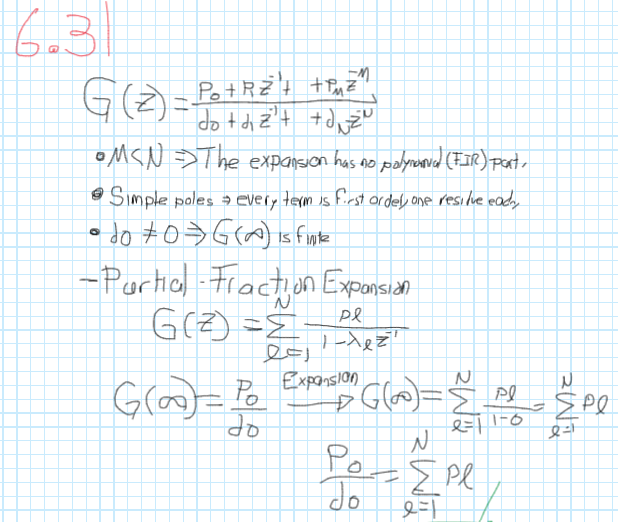
\includegraphics{figures/6_31.png}
\caption{Hand solution, Problem 6.31}
\end{figure}


\subsection{6.47 | Difference equation to H(z), h[n] and s[n]}
A causal LTI discrete-time system is described by the difference equation

\[
y[n] = 0.4\, y[n-1] + 0.05\, y[n-2] + 3\, x[n],
\]
where $x[n]$ and $y[n]$ are, respectively, the input and the output sequences of the system.

(a) Determine the transfer function $H(z)$ of the system.

(b) Determine the impulse response $h[n]$ of the system.

(c) Determine the step response $s[n]$ of the system.

\emph{Method.} For (a), transform the difference equation term by term using linearity and the time-shifting property with zero initial conditions (Sec. 6.7.2, p. 309; Table 6.2, p. 297), then factor the denominator by multiplying through by $z^2$. Both poles turn out to lie inside the unit circle, so the system is causal and stable (Sec. 6.7.5, p. 315). For (b), invert by partial fractions (Sec. 6.4.3, p. 291). For (c), use the convolution theorem with $\mu[n] \leftrightarrow 1/(1 - z^{-1})$ (Table 6.1, p. 281), so $S(z) = H(z)/(1 - z^{-1})$. Useful checks: $h[0]$ must equal $H(\infty)$, $s[0]$ must equal $h[0]$, and $s[\infty]$ must equal the dc gain $H(1)$.

\begin{figure}[H]
\centering
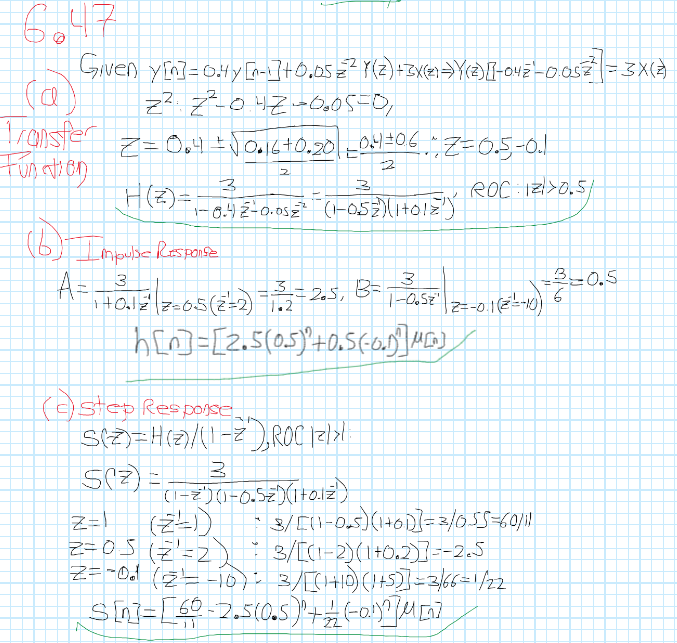
\includegraphics{figures/6_47.png}
\caption{Hand solution, Problem 6.47}
\end{figure}


\subsection{6.59 | Length-4 FIR from three frequency samples}
The frequency response $H(e^{j\omega})$ of a length-4 FIR filter with a real impulse response has the following specific values:

\[
H(e^{j0}) = 2, \qquad H(e^{j\pi/2}) = 7 - j3, \qquad H(e^{j\pi}) = 0 .
\]
Determine $H(z)$.

\emph{Method.} Write $H(e^{j\omega}) = h_0 + h_1 e^{-j\omega} + h_2 e^{-j2\omega} + h_3 e^{-j3\omega}$ (Sec. 6.7.3, p. 312) and evaluate it at the three given frequencies. Because $h[n]$ is real, the DTFT is conjugate symmetric, $H(e^{-j\omega}) = H^{*}(e^{j\omega})$, so $H$ is real at $\omega = 0$ and at $\omega = \pi$; each of those gives one real equation, while $\omega = \pi/2$ gives two (real and imaginary parts). That is four equations for the four unknowns $h_0, h_1, h_2, h_3$. Adding and subtracting the $\omega = 0$ and $\omega = \pi$ equations decouples the system.

\begin{figure}[H]
\centering
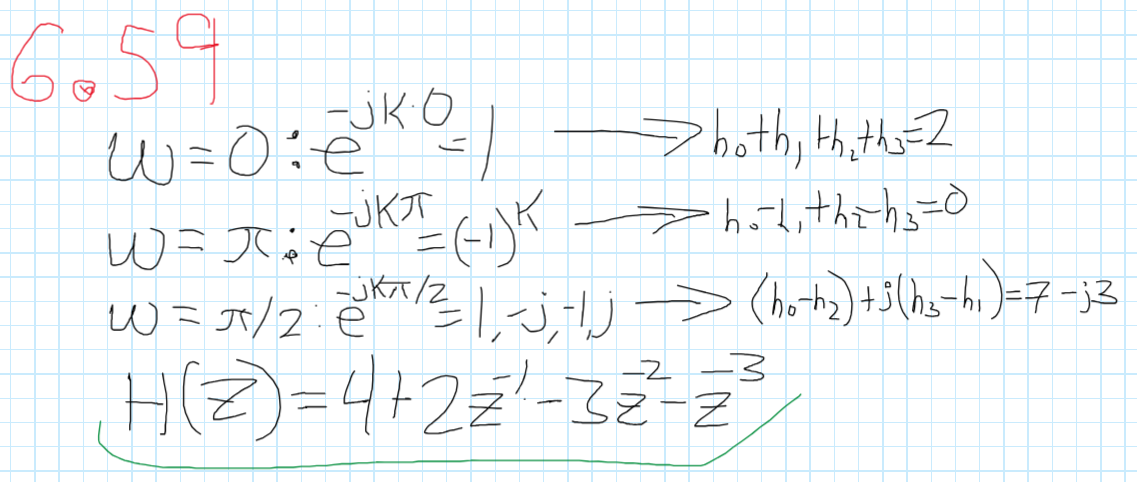
\includegraphics{figures/6_59.png}
\caption{Hand solution, Problem 6.59}
\end{figure}


\subsection{6.81 | ROCs, stability, causality and the form of h[n]}
The transfer function of an LTI discrete-time system is given by

\[
H(z) = \frac{3(z + 1.8)(z - 4)}{(z + 0.3)(z - 0.6)(z + 5)} .
\]
(a) Does the frequency response $H(e^{j\omega})$ of the system exist? Justify your answer.

(b) Can the system be stable? If it is stable, can it be causal?

(c) Determine the form of its impulse response $h[n]$ without evaluating the inverse $z$-transform of $H(z)$.

\emph{Method.} List the poles and their magnitudes; the ROC must be one of the annuli they bound (Sec. 6.3, p. 283). For (a), the frequency response is $H(z)$ evaluated on $|z| = 1$, so it exists if and only if the ROC contains the unit circle (Sec. 6.7.3, p. 312). For (b), BIBO stability is equivalent to the ROC containing the unit circle, while causality requires the ROC to be the exterior of the outermost pole (Sec. 6.7.5, p. 315); check whether both can hold at once. For (c), split the poles according to which side of the chosen annulus they fall on: those inside the inner radius give right-sided terms, those outside the outer radius give left-sided terms. Note also that expanding $H(z)/z$ introduces a pole at $z = 0$, which contributes a $\delta[n]$ term with coefficient $H(0)$.

\begin{figure}[H]
\centering
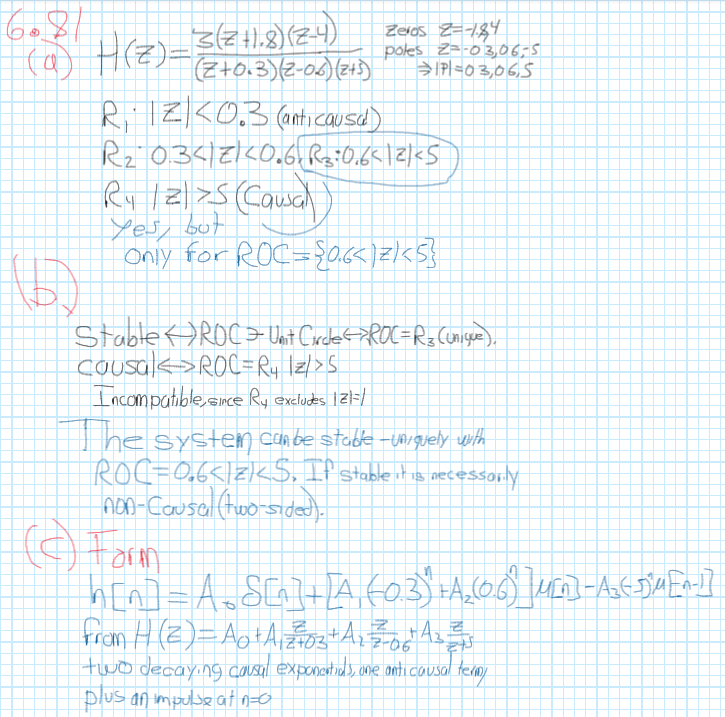
\includegraphics{figures/6_81.png}
\caption{Hand solution, Problem 6.81}
\end{figure}




\end{document}
